\documentclass{article}
\usepackage[utf8]{inputenc}
\usepackage{graphicx}
\usepackage{tabularx}
\usepackage{amsmath}
\usepackage{amsfonts}
\usepackage{amssymb}
\usepackage{pgfplots}
\pgfplotsset{compat=1.17}
\usepackage{subcaption} % Required for subfigures/subtables
\usepackage{hyperref} % Added
\usepackage{url} % Added
\usepackage{microtype}
\usepackage{booktabs}
\usepackage{float} % For [H] exact float placement
\usepackage{colortbl} % For \cellcolor

\usepackage[margin=2.5cm]{geometry}
\usepackage{fancyhdr}
\usepackage{xcolor}

% Define Professional Colors
\definecolor{SeverityCritical}{HTML}{8B0000} % Dark Red
\definecolor{SeverityHigh}{HTML}{E65100}     % Dark Orange
\definecolor{SeverityMedium}{HTML}{FFB300}   % Amber
\definecolor{SeverityLow}{HTML}{1976D2}      % Blue
\definecolor{SeverityUnknown}{HTML}{757575}  % Grey

\pagestyle{fancy}
\fancyhf{}
\rhead{\footnotesize OpenBao Security Evolution Analysis}
\lhead{\footnotesize v2.4.0 to v2.7.0}
\rfoot{\footnotesize Page \thepage}
\lfoot{\footnotesize \today}

\hypersetup{ % Added
    pdftitle={OpenBao Security Evolution Analysis Report (v2.4.0 to v2.7.0)},
    pdfauthor={Adrien SALES, geol, Trivy and Claude Code},
    pdfsubject={Security Evolution and Vulnerability Analysis of OpenBao Versions v2.4.0 to v2.7.0},
    pdfkeywords={OpenBao, Vulnerability, Trivy, Geol, Claude Code, Security, OCI Images},
    colorlinks=true,
    linkcolor=SeverityLow,
    citecolor=SeverityLow,
    urlcolor=SeverityLow,
    breaklinks=true,
}

\title{\textbf{OpenBao Security Evolution Analysis Report} \\ \large Versions 2.4.0 to 2.7.0}
\author{Adrien SALES, geol, Trivy and Claude Code}
\date{\today}

\begin{document}

\maketitle

\begin{abstract}
This document provides a comprehensive analysis of the security evolution in OpenBao, covering major and minor releases from version 2.4.0 to 2.7.0.

Utilizing the Trivy vulnerability scanner on the respective OCI images, this report highlights the continuous improvement in the security posture of the project. To ensure a methodologically sound comparison, \textbf{all fifteen image versions were rescanned in a single session against an identical Trivy vulnerability database}, eliminating the database-drift bias that arises when versions are scanned weeks apart. The analysis encompasses vulnerability trends by severity and provides insights into the impact of base image updates (Alpine Linux) on the overall risk profile. The findings demonstrate a significant and consistent reduction in critical and high-severity vulnerabilities, validating the project's commitment to security and the importance of adopting the latest stable releases.
\end{abstract}

\clearpage

\section{Executive Summary}

\subsection{Key Security Metrics at a Glance}

\noindent
\begin{minipage}[t]{0.24\textwidth}
    \colorbox{SeverityCritical!20}{%
        \begin{minipage}{\linewidth}
            \centering
            \vspace{0.3cm}
            {\large \textbf{Critical}}\\[0.2cm]
            {\Huge \textcolor{SeverityCritical}{\textbf{0}}}\\[0.1cm]
            {\small v2.7.0}\\[0.1cm]
            {\footnotesize \textcolor{gray}{(was 9 in v2.4.0)}}\\
            \vspace{0.3cm}
        \end{minipage}
    }
\end{minipage}%
\hfill
\begin{minipage}[t]{0.24\textwidth}
    \colorbox{SeverityHigh!20}{%
        \begin{minipage}{\linewidth}
            \centering
            \vspace{0.3cm}
            {\large \textbf{High}}\\[0.2cm]
            {\Huge \textcolor{SeverityHigh}{\textbf{0}}}\\[0.1cm]
            {\small v2.7.0}\\[0.1cm]
            {\footnotesize \textcolor{gray}{(was 79 in v2.4.0)}}\\
            \vspace{0.3cm}
        \end{minipage}
    }
\end{minipage}%
\hfill
\begin{minipage}[t]{0.24\textwidth}
    \colorbox{SeverityMedium!20}{%
        \begin{minipage}{\linewidth}
            \centering
            \vspace{0.3cm}
            {\large \textbf{Medium}}\\[0.2cm]
            {\Huge \textcolor{SeverityMedium}{\textbf{0}}}\\[0.1cm]
            {\small v2.7.0}\\[0.1cm]
            {\footnotesize \textcolor{gray}{(was 79 in v2.4.0)}}\\
            \vspace{0.3cm}
        \end{minipage}
    }
\end{minipage}%
\hfill
\begin{minipage}[t]{0.24\textwidth}
    \colorbox{SeverityLow!20}{%
        \begin{minipage}{\linewidth}
            \centering
            \vspace{0.3cm}
            {\large \textbf{Low}}\\[0.2cm]
            {\Huge \textcolor{SeverityLow}{\textbf{0}}}\\[0.1cm]
            {\small v2.7.0}\\[0.1cm]
            {\footnotesize \textcolor{gray}{(was 66 in v2.4.0)}}\\
            \vspace{0.3cm}
        \end{minipage}
    }
\end{minipage}

\vspace{0.5cm}

\subsection{Key Takeaways}

\begin{itemize}
    \item \textbf{Lowest Vulnerability Count:} v2.7.0 --- \textbf{1} total finding, 0 Critical/High/Medium/Low, Security Score: \textcolor{green!60!black}{\textbf{100.0/100}} (a perfect weighted score: the single remaining item is Unknown-severity and therefore carries no weight)
    \item \textbf{Highest Vulnerability Count:} v2.4.0/v2.4.1 --- 235 total vulnerabilities, 9 Critical, Security Score: \textcolor{red}{\textbf{0/100}}
    \item \textbf{Biggest Improvement:} v2.6.3 $\rightarrow$ v2.7.0 --- \textbf{88.9\% reduction} (9 $\rightarrow$ 1), as the 2.7.0 release closes every outstanding OpenBao core advisory at once
    \item \textbf{Recommended Minimum:} v2.6.3+ for production use (Score $\geq$ 95.8/100). Because this rescan used a Trivy database four months newer than the previous edition of this report, \textbf{every} version's counts rose against their previously published values (e.g.\ v2.6.1: 10 $\rightarrow$ 47, v2.5.5: 15 $\rightarrow$ 55) --- a textbook illustration of CVE database drift, and the reason all fifteen tags are always rescanned together.
    \item \textbf{Overall Improvement:} \textbf{99.6\% reduction} from v2.4.0 to v2.7.0 (235 $\rightarrow$ 1 vulnerabilities)
    \item \textbf{Latest Version:} v2.7.0 --- The first release in this series with \textbf{no Critical, High, Medium or Low findings at all}. It clears the seven long-standing OpenBao core CVEs (CVE-2024-8185, CVE-2024-9180, CVE-2025-59043, CVE-2025-64761, CVE-2026-45808, CVE-2026-46358, CVE-2026-46405) that had persisted in all fourteen prior releases, and inherits the Alpine 3.24.2 base introduced in v2.6.3 that zeroes the OS layer.
    \item \textbf{Vulnerability Remediation:} 97--99\% of CVEs are fixable across v2.4.0--v2.6.2. v2.6.3 drops to 89\% and v2.7.0 to 0\%, but this is a sign of health, not risk: as the fixable backlog is cleared, the only finding left is GO-2026-5932, an advisory on the unmaintained \texttt{golang.org/x/crypto/openpgp} package for which no upstream fix exists.
    \item \textbf{Versioning Policy:} OpenBao follows Semantic Versioning. Upgrading from v2.5.x to v2.5.y is \textbf{strongly encouraged} and considered low-risk. These updates are essential to benefit from security patches, bug fixes, and performance improvements without breaking compatibility. Staying on the latest patch of a minor release is the recommended security best practice.
\end{itemize}

\subsection{Security Posture Scores}

The Security Posture Score provides a normalized risk assessment based on weighted severity levels (Critical: 10 points, High: 5 points, Medium: 2 points, Low: 1 point). Scores range from 0 (highest risk) to 100 (lowest risk).

\begin{table}[H]
    \centering
    \caption{Security Posture Score by Version}
    \label{tab:security_scores}
    \begin{tabularx}{\textwidth}{l*{5}{>{\centering\arraybackslash}X}l}
        \toprule
        \textbf{Version} & \textbf{Critical} & \textbf{High} & \textbf{Medium} & \textbf{Low} & \textbf{Total} & \textbf{Score /100} \\
        \midrule
        2.4.0 & 9  & 79 & 79 & 66 & 233 & \textcolor{red}{\textbf{0.0}} \\
        2.4.1 & 9  & 79 & 79 & 66 & 233 & \textcolor{red}{\textbf{0.0}} \\
        2.4.3 & 9  & 78 & 62 & 63 & 212 & \textcolor{red}{6.0} \\
        2.4.4 & 9  & 78 & 60 & 63 & 210 & \textcolor{red}{6.5} \\
        2.5.0 & 9  & 71 & 48 & 44 & 172 & \textcolor{red}{17.5} \\
        2.5.1 & 8  & 70 & 48 & 44 & 170 & \textcolor{red}{19.7} \\
        2.5.2 & 6  & 69 & 47 & 42 & 164 & \textcolor{orange}{23.7} \\
        2.5.3 & 1  & 45 & 36 & 37 & 119 & \textcolor{orange}{51.5} \\
        2.5.4 & 1  & 39 & 33 & 37 & 110 & \textcolor{orange}{56.6} \\
        2.5.5 & 1  & 23 & 15 & 15 & 54  & \textcolor{green!60!black}{\textbf{76.1}} \\
        2.6.0 & 0  & 22 & 13 & 13 & 48  & \textcolor{green!60!black}{\textbf{79.0}} \\
        2.6.1 & 0  & 20 & 13 & 13 & 46  & \textcolor{green!60!black}{\textbf{80.4}} \\
        2.6.2 & 0  & 11 & 12 & 13 & 36  & \textcolor{green!60!black}{\textbf{87.1}} \\
        2.6.3 & 0  & 5  & 2  & 1  & 8   & \textcolor{green!60!black}{\textbf{95.8}} \\
        2.7.0 & 0  & 0  & 0  & 0  & 0   & \textcolor{green!60!black}{\textbf{100.0}} \\
        \bottomrule
    \end{tabularx}
\end{table}

\subsection{Risk Level Matrix}

This matrix provides a quick visual assessment of the risk level associated with each version based on vulnerability composition.

\begin{table}[H]
    \centering
    \caption{Risk Level Assessment by Version}
    \label{tab:risk_matrix}
    \begin{tabularx}{\textwidth}{l*{4}{>{\centering\arraybackslash}X}l}
        \toprule
        \textbf{Version} & \textbf{Critical} & \textbf{High} & \textbf{Medium} & \textbf{Low} & \textbf{Risk Level} \\
        \midrule
        2.4.0 & \cellcolor{SeverityCritical!40}9 & \cellcolor{SeverityHigh!40}79 & \cellcolor{SeverityMedium!40}79 & \cellcolor{SeverityLow!40}66 & \textcolor{red}{\textbf{HIGH}} \\
        2.4.1 & \cellcolor{SeverityCritical!40}9 & \cellcolor{SeverityHigh!40}79 & \cellcolor{SeverityMedium!40}79 & \cellcolor{SeverityLow!40}66 & \textcolor{red}{\textbf{HIGH}} \\
        2.4.3 & \cellcolor{SeverityCritical!40}9 & \cellcolor{SeverityHigh!40}78 & \cellcolor{SeverityMedium!40}62 & \cellcolor{SeverityLow!40}63 & \textcolor{red}{\textbf{HIGH}} \\
        2.4.4 & \cellcolor{SeverityCritical!40}9 & \cellcolor{SeverityHigh!40}78 & \cellcolor{SeverityMedium!40}60 & \cellcolor{SeverityLow!40}63 & \textcolor{red}{\textbf{HIGH}} \\
        2.5.0 & \cellcolor{SeverityCritical!40}9 & \cellcolor{SeverityHigh!30}71 & \cellcolor{SeverityMedium!30}48 & \cellcolor{SeverityLow!30}44 & \textcolor{red}{\textbf{HIGH}} \\
        2.5.1 & \cellcolor{SeverityCritical!40}8 & \cellcolor{SeverityHigh!30}70 & \cellcolor{SeverityMedium!30}48 & \cellcolor{SeverityLow!30}44 & \textcolor{red}{\textbf{HIGH}} \\
        2.5.2 & \cellcolor{SeverityCritical!20}6 & \cellcolor{SeverityHigh!30}69 & \cellcolor{SeverityMedium!30}47 & \cellcolor{SeverityLow!30}42 & \textcolor{orange}{\textbf{MEDIUM}} \\
        2.5.3 & \cellcolor{SeverityCritical!10}1 & \cellcolor{SeverityHigh!20}45 & \cellcolor{SeverityMedium!20}36 & \cellcolor{SeverityLow!20}37 & \textcolor{orange}{\textbf{MEDIUM}} \\
        2.5.4 & \cellcolor{SeverityCritical!10}1 & \cellcolor{SeverityHigh!15}39 & \cellcolor{SeverityMedium!15}33 & \cellcolor{SeverityLow!15}37 & \textcolor{orange}{\textbf{MEDIUM}} \\
        2.5.5 & \cellcolor{SeverityCritical!10}1 & \cellcolor{SeverityHigh!10}23 & \cellcolor{SeverityMedium!10}15 & \cellcolor{SeverityLow!10}15 & \textcolor{green!60!black}{\textbf{LOW}} \\
        2.6.0 & \cellcolor{white}0                & \cellcolor{SeverityHigh!10}22 & \cellcolor{SeverityMedium!10}13 & \cellcolor{SeverityLow!10}13 & \textcolor{green!60!black}{\textbf{LOW}} \\
        2.6.1 & \cellcolor{white}0                & \cellcolor{SeverityHigh!10}20 & \cellcolor{SeverityMedium!10}13 & \cellcolor{SeverityLow!10}13 & \textcolor{green!60!black}{\textbf{LOW}} \\
        2.6.2 & \cellcolor{white}0                & \cellcolor{SeverityHigh!10}11 & \cellcolor{SeverityMedium!10}12 & \cellcolor{SeverityLow!10}13 & \textcolor{green!60!black}{\textbf{LOW}} \\
        2.6.3 & \cellcolor{white}0                & \cellcolor{SeverityHigh!10}5 & \cellcolor{SeverityMedium!10}2 & \cellcolor{SeverityLow!10}1 & \textcolor{green!60!black}{\textbf{LOW}} \\
        2.7.0 & \cellcolor{white}0                & \cellcolor{white}0                & \cellcolor{white}0                & \cellcolor{white}0                & \textcolor{green!60!black}{\textbf{LOW}} \\
        \bottomrule
    \end{tabularx}
\end{table}

\textbf{Risk Level Guidelines:}
\begin{itemize}
    \item \textcolor{red}{\textbf{HIGH}} (Score $<$ 20): Not recommended for production. Contains critical vulnerabilities requiring immediate attention.
    \item \textcolor{orange}{\textbf{MEDIUM}} (Score 20-70): Use with caution. Suitable for development environments with proper monitoring.
    \item \textcolor{green!60!black}{\textbf{LOW}} (Score $>$ 70): Recommended for production. Minimal security concerns with available patches.
\end{itemize}

\clearpage

\section{Introduction}
This report provides an in-depth analysis of the security evolution in OpenBao from version 2.4.0 through 2.7.0. The assessment was performed using the Trivy vulnerability scanner on the official OCI images for each release. The primary objective is to track the evolution of the project's security posture over time, identifying trends in vulnerability counts across different severity levels and evaluating the impact of maintenance and updates, such as base operating system upgrades.

\subsection{OpenBao Versioning Policy and Release Strategy}
OpenBao adheres to \textbf{Semantic Versioning} principles, ensuring predictable and transparent release management. The project follows a versioning scheme similar to industry standards, where version numbers follow the pattern \texttt{MAJOR.MINOR.PATCH}.

Similar to PostgreSQL's versioning policy\footnote{PostgreSQL Versioning Policy: \url{https://www.postgresql.org/support/versioning/}}, OpenBao's minor releases are designed to be \textbf{low-risk updates} that focus on:

\begin{itemize}
    \item Fixes for frequently-encountered bugs
    \item Low-risk stability improvements
    \item Security vulnerability patches
    \item Data corruption prevention
\end{itemize}

\textbf{The OpenBao community considers performing minor upgrades to be less risky than continuing to run an old minor version.} This philosophy is validated by the security analysis presented in this report, where consistent minor version updates demonstrate significant vulnerability reduction without introducing breaking changes.

As PostgreSQL documentation states: \textit{``Minor releases only contain fixes for frequently-encountered bugs, low-risk fixes, security issues, and data corruption problems. The community considers performing minor upgrades to be less risky than continuing to run an old minor version.''} This same principle applies to OpenBao's release strategy, making the adoption of latest minor releases a recommended security best practice.

\section{Tooling Details}
This comparative analysis report was generated and compiled using several tools, including an AI agent (Claude Code), to assess and present the vulnerability data.

\subsection{Claude Code}
This entire report, including the analysis, data extraction, and LaTeX document generation, was orchestrated by an instance of Claude Code. The agent was responsible for:
\begin{enumerate}
    \item Interacting with vulnerability scanning tools.
    \item Parsing their outputs.
    \item Performing comparative data analysis.
    \item Constructing the LaTeX document structure.
    \item Generating the textual content and charts.
    \item Compiling the \LaTeX{} document into a PDF.
    \item Obtaining End-of-Life (EOL) information for OpenBao versions from Geol.
\end{enumerate}

\subsection{Geol}
Geol is a tool used for providing product lifecycle and support information.
\begin{itemize}
    \item \textbf{Version:} 2.21.4
    \item \textbf{Usage:} Querying OpenBao release lifecycles and support status.
\end{itemize}

\subsection{Trivy}
Trivy (v0.74.0) is a comprehensive security scanner for container images. It was the primary tool for vulnerability assessment in this report. \textbf{All fifteen image tags were rescanned on the same day against a single, shared vulnerability database} (downloaded once with \texttt{--download-db-only}, then reused via \texttt{--skip-db-update}), so that every version is evaluated against the exact same set of known CVEs.
\begin{itemize}
    \item \textbf{Vulnerability Database Updated:} \today{}
    \item \textbf{Scanning Commands Examples:}
    {\small
\begin{verbatim}
trivy image --format json --output openbao_2.4.0.json openbao/openbao:2.4.0
trivy image --format json --output openbao_2.7.0.json openbao/openbao:2.7.0
\end{verbatim}
    }
    \item \textbf{Analyzed Image Tags:} 2.4.0, 2.4.1, 2.4.3, 2.4.4, 2.5.0, 2.5.1, 2.5.2, 2.5.3, 2.5.4, 2.5.5, 2.6.0, 2.6.1, 2.6.2, 2.6.3, 2.7.0.
\end{itemize}

\section{Tool Homepages}
\begin{itemize}
    \item \textbf{Claude Code:} \url{https://claude.com/claude-code}
    \item \textbf{Geol:} \url{https://github.com/opt-nc/geol}
    \item \textbf{Trivy:} \url{https://trivy.dev/}
\end{itemize}

\section{Base Image Analysis}
The security posture of an OCI image is heavily influenced by its base operating system. OpenBao utilizes Alpine Linux, a security-oriented, lightweight Linux distribution based on musl libc and busybox.

\subsection{Base OS Freshness}
Using the newest Alpine patch available is as important as the choice of major/minor branch: Alpine ships synchronized security-patch releases across all supported branches roughly every 4--10 weeks. For each OpenBao release, we cross-referenced \textbf{geol} (Alpine Linux cycle/EOL data) with the exact \textbf{Docker Hub tag publish timestamps} for every \texttt{alpine:3.2x.y} tag to reconstruct which Alpine patch was actually the latest one publicly available on the day each OpenBao image was built --- not merely the latest one known today (the two can differ, since new Alpine patches are released continuously).

\begin{table}[H]
    \centering
    \caption{Base OS Versions (Alpine Linux) and Freshness at Release Time}
    \label{tab:base_images}
    {\small
    \begin{tabularx}{\textwidth}{l l >{\centering\arraybackslash}X >{\centering\arraybackslash}X >{\centering\arraybackslash}X}
        \toprule
        \textbf{OpenBao Version} & \textbf{Base OS} & \textbf{Version Used} & \textbf{Latest Alpine Available (that day)} & \textbf{Latest at Release?} \\
        \midrule
        2.4.0         & Alpine & 3.22.1 & 3.22.1 & \textcolor{green!60!black}{\textbf{Yes}} \\
        2.4.1         & Alpine & 3.22.1 & 3.22.1 & \textcolor{green!60!black}{\textbf{Yes}} \\
        2.4.3         & Alpine & 3.22.2 & 3.22.2 & \textcolor{green!60!black}{\textbf{Yes}} \\
        2.4.4         & Alpine & 3.22.2 & 3.22.2 & \textcolor{green!60!black}{\textbf{Yes}} \\
        2.5.0         & Alpine & 3.23.3 & 3.23.3 & \textcolor{green!60!black}{\textbf{Yes}} \\
        2.5.1         & Alpine & 3.23.3 & 3.23.3 & \textcolor{green!60!black}{\textbf{Yes}} \\
        2.5.2         & Alpine & 3.23.3 & 3.23.3 & \textcolor{green!60!black}{\textbf{Yes}} \\
        2.5.3         & Alpine & 3.23.4 & 3.23.4 & \textcolor{green!60!black}{\textbf{Yes}} \\
        2.5.4         & Alpine & 3.23.4 & 3.23.4 & \textcolor{green!60!black}{\textbf{Yes}} \\
        2.5.5         & Alpine & 3.24.1 & 3.24.1 & \textcolor{green!60!black}{\textbf{Yes}} \\
        2.6.0         & Alpine & 3.24.1 & 3.24.1 & \textcolor{green!60!black}{\textbf{Yes}} \\
        2.6.1         & Alpine & 3.24.1 & 3.24.1 & \textcolor{green!60!black}{\textbf{Yes}} \\
        2.6.2         & Alpine & 3.24.1 & 3.24.1 & \textcolor{green!60!black}{\textbf{Yes}} \\
        2.6.3         & Alpine & 3.24.2 & 3.24.2 & \textcolor{green!60!black}{\textbf{Yes}} \\
        2.7.0         & Alpine & 3.24.2 & 3.24.2 & \textcolor{green!60!black}{\textbf{Yes}} \\
        \bottomrule
    \end{tabularx}
    }
\end{table}

\noindent\textbf{Finding:} every single analyzed OpenBao release --- all fifteen --- shipped with the Alpine patch that was the most recent one publicly available on its build date (e.g.\ v2.5.3 was built 2026-04-20, five days after Alpine 3.23.4 published on 2026-04-15; v2.6.3 and v2.7.0 were both built 2026-09-23, five days after Alpine 3.24.2 published on 2026-09-18). None of the ``stale-looking'' minor-version gaps in Table~\ref{tab:base_images} (e.g.\ v2.6.0, v2.6.1 and v2.6.2 all staying on Alpine 3.24.1) reflect a missed update: in each case, no newer Alpine patch had been published yet at the time of that OpenBao build. This indicates disciplined, continuous base-image rebasing by the OpenBao maintainers rather than periodic/lagging updates.

\section{Security Evolution Analysis (v2.4.0 to v2.7.0)}

\subsection{Vulnerability Evolution Table}
{\small
\begin{table}[H]
    \centering
    \caption{Vulnerability Counts: v2.4.0 through v2.7.0}
    \label{tab:evolution_vulnerability_counts}
    \begin{tabularx}{\textwidth}{l*{5}{>{\centering\arraybackslash}X}}
        \toprule
        \textbf{Version} & \textbf{Critical} & \textbf{High} & \textbf{Medium} & \textbf{Low} & \textbf{Unknown} \\
        \midrule
        2.4.0            & 9                 & 79            & 79              & 66           & 2                \\
        2.4.1            & 9                 & 79            & 79              & 66           & 2                \\
        2.4.3            & 9                 & 78            & 62              & 63           & 2                \\
        2.4.4            & 9                 & 78            & 60              & 63           & 2                \\
        2.5.0            & 9                 & 71            & 48              & 44           & 2                \\
        2.5.1            & 8                 & 70            & 48              & 44           & 2                \\
        2.5.2            & 6                 & 69            & 47              & 42           & 2                \\
        2.5.3            & 1                 & 45            & 36              & 37           & 2                \\
        2.5.4            & 1                 & 39            & 33              & 37           & 2                \\
        2.5.5            & 1                 & 23            & 15              & 15           & 1                \\
        2.6.0            & 0                 & 22            & 13              & 13           & 1                \\
        2.6.1            & 0                 & 20            & 13              & 13           & 1                \\
        2.6.2            & 0                 & 11            & 12              & 13           & 1                \\
        2.6.3            & 0                 & 5             & 2               & 1            & 1                \\
        2.7.0            & 0                 & 0             & 0               & 0            & 1                \\
        \bottomrule
    \end{tabularx}
\end{table}
}

\subsection{Overall Security Trend Chart}
\begin{figure}[H]
    \centering
    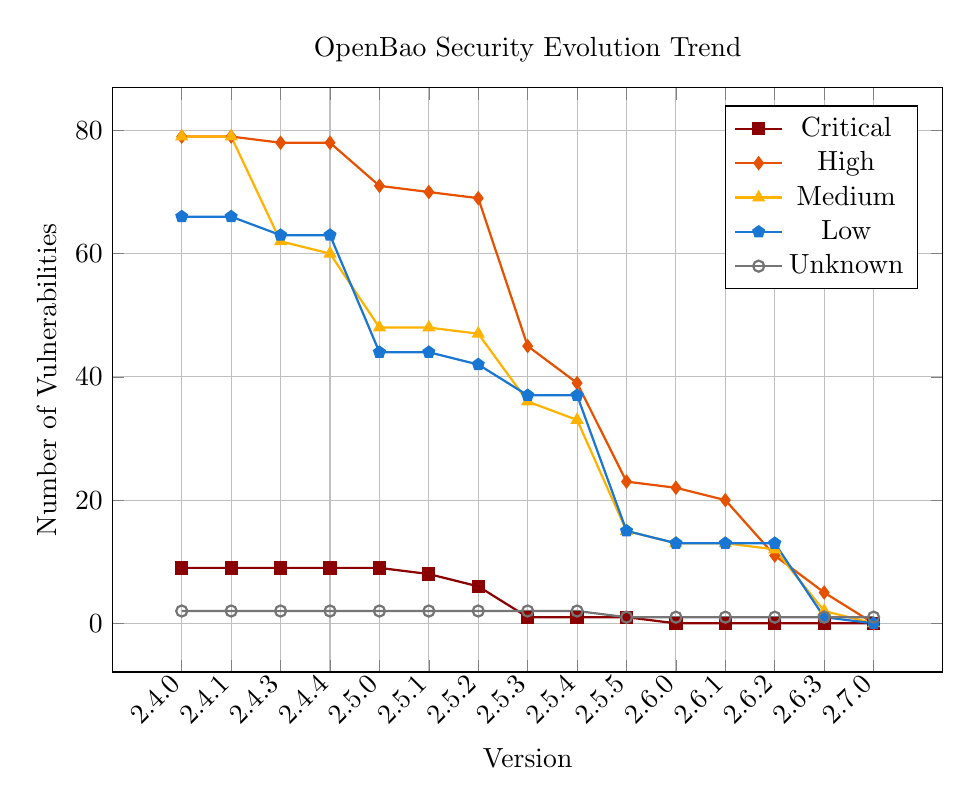
\begin{tikzpicture}
        \begin{axis}[
            title={OpenBao Security Evolution Trend},
            xlabel={Version},
            ylabel={Number of Vulnerabilities},
            symbolic x coords={2.4.0,2.4.1,2.4.3,2.4.4,2.5.0,2.5.1,2.5.2,2.5.3,2.5.4,2.5.5,2.6.0,2.6.1,2.6.2,2.6.3,2.7.0},
            xtick=data,
            x tick label style={rotate=45,anchor=east},
            legend pos=north east,
            grid=major,
            width=\textwidth,
            height=9cm,
        ]
        \addplot[color=SeverityCritical,thick,mark=square*] coordinates {
            (2.4.0,9) (2.4.1,9) (2.4.3,9) (2.4.4,9) (2.5.0,9) (2.5.1,8) (2.5.2,6) (2.5.3,1) (2.5.4,1) (2.5.5,1) (2.6.0,0) (2.6.1,0) (2.6.2,0) (2.6.3,0) (2.7.0,0)
        };
        \addplot[color=SeverityHigh,thick,mark=diamond*] coordinates {
            (2.4.0,79) (2.4.1,79) (2.4.3,78) (2.4.4,78) (2.5.0,71) (2.5.1,70) (2.5.2,69) (2.5.3,45) (2.5.4,39) (2.5.5,23) (2.6.0,22) (2.6.1,20) (2.6.2,11) (2.6.3,5) (2.7.0,0)
        };
        \addplot[color=SeverityMedium,thick,mark=triangle*] coordinates {
            (2.4.0,79) (2.4.1,79) (2.4.3,62) (2.4.4,60) (2.5.0,48) (2.5.1,48) (2.5.2,47) (2.5.3,36) (2.5.4,33) (2.5.5,15) (2.6.0,13) (2.6.1,13) (2.6.2,12) (2.6.3,2) (2.7.0,0)
        };
        \addplot[color=SeverityLow,thick,mark=pentagon*] coordinates {
            (2.4.0,66) (2.4.1,66) (2.4.3,63) (2.4.4,63) (2.5.0,44) (2.5.1,44) (2.5.2,42) (2.5.3,37) (2.5.4,37) (2.5.5,15) (2.6.0,13) (2.6.1,13) (2.6.2,13) (2.6.3,1) (2.7.0,0)
        };
        \addplot[color=SeverityUnknown,thick,mark=o] coordinates {
            (2.4.0,2) (2.4.1,2) (2.4.3,2) (2.4.4,2) (2.5.0,2) (2.5.1,2) (2.5.2,2) (2.5.3,2) (2.5.4,2) (2.5.5,1) (2.6.0,1) (2.6.1,1) (2.6.2,1) (2.6.3,1) (2.7.0,1)
        };
        \legend{Critical, High, Medium, Low, Unknown}
        \end{axis}
    \end{tikzpicture}
    \caption{Security Improvement Trend: v2.4.0 to v2.7.0}
    \label{fig:overall_evolution}
\end{figure}

\subsection{Stacked Area Chart: Total Vulnerability Composition}
This stacked area chart provides a complementary view of the security evolution, showing the total volume and composition of vulnerabilities by severity level.

\begin{figure}[H]
    \centering
    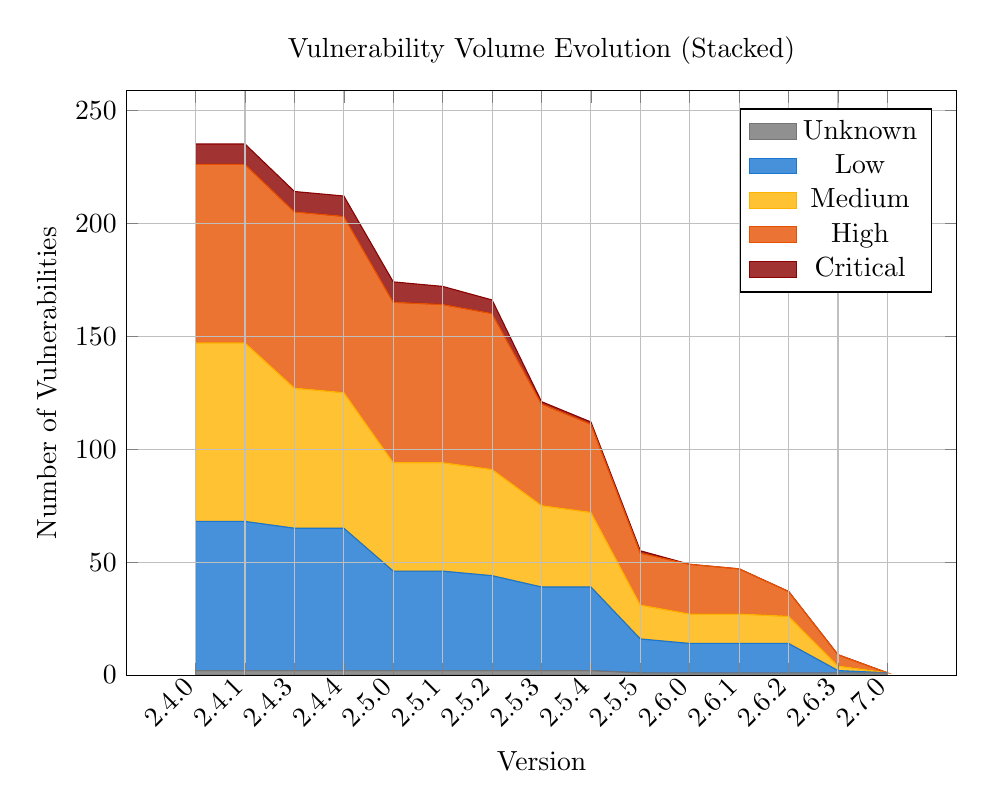
\begin{tikzpicture}
        \begin{axis}[
            title={Vulnerability Volume Evolution (Stacked)},
            xlabel={Version},
            ylabel={Number of Vulnerabilities},
            symbolic x coords={2.4.0,2.4.1,2.4.3,2.4.4,2.5.0,2.5.1,2.5.2,2.5.3,2.5.4,2.5.5,2.6.0,2.6.1,2.6.2,2.6.3,2.7.0},
            xtick=data,
            x tick label style={rotate=45,anchor=east},
            legend pos=north east,
            grid=major,
            width=\textwidth,
            height=9cm,
            ymin=0,
            stack plots=y,
            area style,
        ]
        \addplot+[color=SeverityUnknown,fill=SeverityUnknown,fill opacity=0.8] coordinates {
            (2.4.0,2) (2.4.1,2) (2.4.3,2) (2.4.4,2) (2.5.0,2) (2.5.1,2) (2.5.2,2) (2.5.3,2) (2.5.4,2) (2.5.5,1) (2.6.0,1) (2.6.1,1) (2.6.2,1) (2.6.3,1) (2.7.0,1)
        } \closedcycle;
        \addplot+[color=SeverityLow,fill=SeverityLow,fill opacity=0.8] coordinates {
            (2.4.0,66) (2.4.1,66) (2.4.3,63) (2.4.4,63) (2.5.0,44) (2.5.1,44) (2.5.2,42) (2.5.3,37) (2.5.4,37) (2.5.5,15) (2.6.0,13) (2.6.1,13) (2.6.2,13) (2.6.3,1) (2.7.0,0)
        } \closedcycle;
        \addplot+[color=SeverityMedium,fill=SeverityMedium,fill opacity=0.8] coordinates {
            (2.4.0,79) (2.4.1,79) (2.4.3,62) (2.4.4,60) (2.5.0,48) (2.5.1,48) (2.5.2,47) (2.5.3,36) (2.5.4,33) (2.5.5,15) (2.6.0,13) (2.6.1,13) (2.6.2,12) (2.6.3,2) (2.7.0,0)
        } \closedcycle;
        \addplot+[color=SeverityHigh,fill=SeverityHigh,fill opacity=0.8] coordinates {
            (2.4.0,79) (2.4.1,79) (2.4.3,78) (2.4.4,78) (2.5.0,71) (2.5.1,70) (2.5.2,69) (2.5.3,45) (2.5.4,39) (2.5.5,23) (2.6.0,22) (2.6.1,20) (2.6.2,11) (2.6.3,5) (2.7.0,0)
        } \closedcycle;
        \addplot+[color=SeverityCritical,fill=SeverityCritical,fill opacity=0.8] coordinates {
            (2.4.0,9) (2.4.1,9) (2.4.3,9) (2.4.4,9) (2.5.0,9) (2.5.1,8) (2.5.2,6) (2.5.3,1) (2.5.4,1) (2.5.5,1) (2.6.0,0) (2.6.1,0) (2.6.2,0) (2.6.3,0) (2.7.0,0)
        } \closedcycle;
        \legend{Unknown, Low, Medium, High, Critical}
        \end{axis}
    \end{tikzpicture}
    \caption{Stacked view showing total vulnerability volume and severity composition}
    \label{fig:stacked_evolution}
\end{figure}

\subsection{Version-to-Version Improvement Rate}
The following table quantifies the percentage reduction in total vulnerabilities between consecutive releases, highlighting the most impactful updates.

\begin{table}[H]
    \centering
    \caption{Vulnerability Reduction Rate Between Versions}
    \label{tab:reduction_rate}
    \begin{tabularx}{\textwidth}{l*{3}{>{\centering\arraybackslash}X}}
        \toprule
        \textbf{Version Transition} & \textbf{Before} & \textbf{After} & \textbf{Reduction} \\
        \midrule
        2.4.0 $\rightarrow$ 2.4.1 & 235 & 235 & 0.0\% \\
        2.4.1 $\rightarrow$ 2.4.3 & 235 & 214 & 8.9\% \\
        2.4.3 $\rightarrow$ 2.4.4 & 214 & 212 & 0.9\% \\
        2.4.4 $\rightarrow$ 2.5.0 & 212 & 174 & 17.9\% \\
        2.5.0 $\rightarrow$ 2.5.1 & 174 & 172 & 1.1\% \\
        2.5.1 $\rightarrow$ 2.5.2 & 172 & 166 & 3.5\% \\
        2.5.2 $\rightarrow$ 2.5.3 & 166 & 121 & \textbf{27.1\%} \\
        2.5.3 $\rightarrow$ 2.5.4 & 121 & 112 & 7.4\% \\
        2.5.4 $\rightarrow$ 2.5.5 & 112 & 55  & \textbf{50.9\%} \\
        2.5.5 $\rightarrow$ 2.6.0 & 55  & 49  & 10.9\% \\
        2.6.0 $\rightarrow$ 2.6.1 & 49  & 47  & 4.1\% \\
        2.6.1 $\rightarrow$ 2.6.2 & 47  & 37  & \textbf{21.3\%} \\
        2.6.2 $\rightarrow$ 2.6.3 & 37  & 9   & \textbf{75.7\%} \\
        2.6.3 $\rightarrow$ 2.7.0 & 9   & 1   & \textbf{88.9\%} \\
        \bottomrule
    \end{tabularx}
\end{table}

The data reveals five major security milestones:
\begin{itemize}
    \item \textbf{v2.5.3:} 27.1\% reduction - Alpine 3.23.4 rebase plus a large application-layer cut (Critical drops from 6 to 1)
    \item \textbf{v2.5.5:} 50.9\% reduction - Alpine upgrade to 3.24.1 more than halves the OS layer (50 $\rightarrow$ 20)
    \item \textbf{v2.6.2:} 21.3\% reduction - Application-layer hardening on the same Alpine 3.24.1 base (27 $\rightarrow$ 17 Go findings), notably halving the High count from 20 to 11
    \item \textbf{v2.6.3:} 75.7\% reduction - The Alpine 3.24.2 rebase \textbf{eliminates all remaining OS-layer vulnerabilities} (20 $\rightarrow$ 0), clearing the OpenSSL \texttt{libcrypto3}/\texttt{libssl3} cluster in a single step
    \item \textbf{v2.7.0:} 88.9\% reduction - The minor release closes every outstanding OpenBao core advisory, leaving a single unfixable Unknown-severity item and a perfect 100.0/100 weighted score
\end{itemize}

\section{Deep Security Insights}
This section provides a more granular analysis of the vulnerability data, distinguishing between different layers of the container image and identifying persistent risks.

\subsection{OS vs. Application Vulnerabilities}
Distinguishing between vulnerabilities in the base operating system (Alpine Linux) and the application layer (Go binaries and dependencies) is crucial for identifying the primary source of risk.

\begin{table}[H]
    \centering
    \caption{Vulnerability Distribution: OS Layer vs. Application Layer}
    \label{tab:os_vs_app}
    \begin{tabularx}{\textwidth}{l*{3}{>{\centering\arraybackslash}X}}
        \toprule
        \textbf{Version} & \textbf{OS (Alpine)} & \textbf{Application (Go)} & \textbf{Total} \\
        \midrule
        2.4.0            & 111 & 124 & 235 \\
        2.4.1            & 111 & 124 & 235 \\
        2.4.3            & 105 & 109 & 214 \\
        2.4.4            & 105 & 107 & 212 \\
        2.5.0            & 75  & 99  & 174 \\
        2.5.1            & 75  & 97  & 172 \\
        2.5.2            & 75  & 91  & 166 \\
        2.5.3            & 50  & 71  & 121 \\
        2.5.4            & 50  & 62  & 112 \\
        2.5.5            & 20  & 35  & 55  \\
        2.6.0            & 20  & 29  & 49  \\
        2.6.1            & 20  & 27  & 47  \\
        2.6.2            & 20  & 17  & 37  \\
        2.6.3            & 0   & 9   & 9   \\
        2.7.0            & 0   & 1   & 1   \\
        \bottomrule
    \end{tabularx}
\end{table}

\begin{figure}[H]
    \centering
    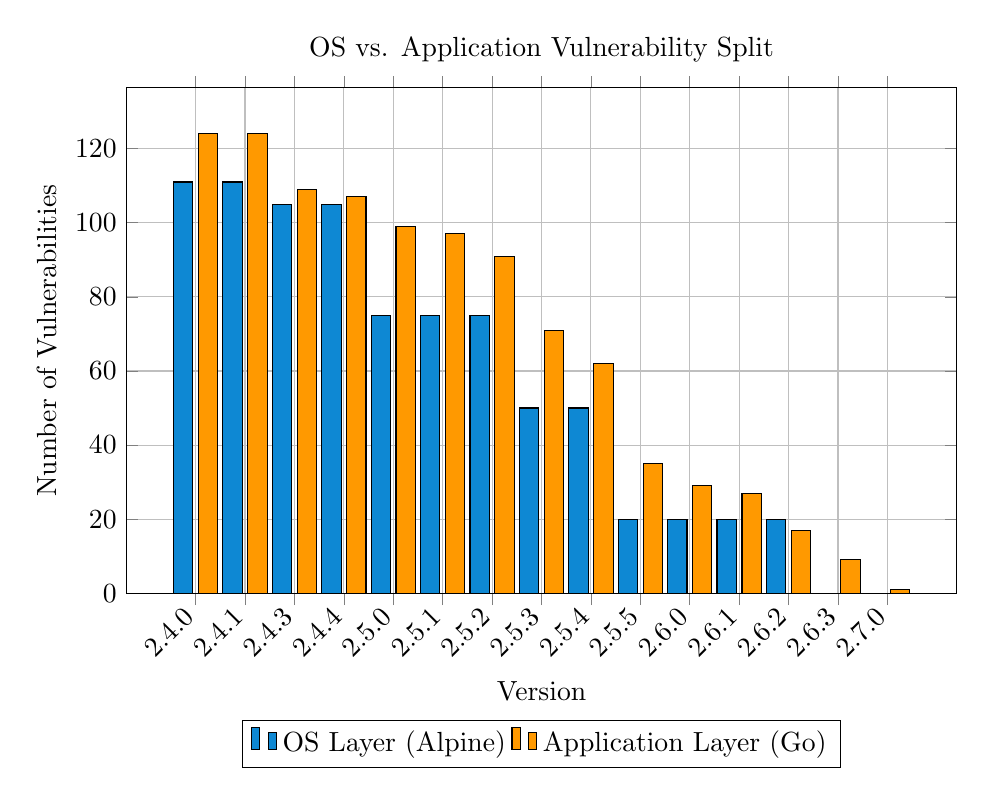
\begin{tikzpicture}
        \begin{axis}[
            ybar,
            title={OS vs. Application Vulnerability Split},
            xlabel={Version},
            ylabel={Number of Vulnerabilities},
            symbolic x coords={2.4.0,2.4.1,2.4.3,2.4.4,2.5.0,2.5.1,2.5.2,2.5.3,2.5.4,2.5.5,2.6.0,2.6.1,2.6.2,2.6.3,2.7.0},
            xtick=data,
            x tick label style={rotate=45,anchor=east},
            legend style={at={(0.5,-0.25)}, anchor=north, legend columns=-1},
            grid=major,
            width=\textwidth,
            height=8cm,
            ymin=0,
            bar width=7pt,
        ]
        \addplot[fill=cyan!70!blue, draw=black] coordinates {
            (2.4.0,111) (2.4.1,111) (2.4.3,105) (2.4.4,105) (2.5.0,75) (2.5.1,75) (2.5.2,75) (2.5.3,50) (2.5.4,50) (2.5.5,20) (2.6.0,20) (2.6.1,20) (2.6.2,20) (2.6.3,0) (2.7.0,0)
        };
        \addplot[fill=orange!80!yellow, draw=black] coordinates {
            (2.4.0,124) (2.4.1,124) (2.4.3,109) (2.4.4,107) (2.5.0,99) (2.5.1,97) (2.5.2,91) (2.5.3,71) (2.5.4,62) (2.5.5,35) (2.6.0,29) (2.6.1,27) (2.6.2,17) (2.6.3,9) (2.7.0,1)
        };
        \legend{OS Layer (Alpine), Application Layer (Go)}
        \end{axis}
    \end{tikzpicture}
    \caption{Visualizing the migration of risk from OS to Application layer}
    \label{fig:os_vs_app_chart}
\end{figure}

The data highlights a decisive milestone in version 2.6.3, where all remaining operating-system vulnerabilities were eliminated (down from 20 in v2.6.2) by the Alpine 3.24.2 rebase --- which cleared an entire cluster of OpenSSL \texttt{libcrypto3}/\texttt{libssl3} advisories (CVE-2026-14456, CVE-2026-18798, CVE-2026-63072--63076, CVE-2026-75803 and others). The OS layer declines steadily across the series: 111 (v2.4.0) $\rightarrow$ 75 (v2.5.0--v2.5.2) $\rightarrow$ 50 (v2.5.3/v2.5.4) $\rightarrow$ 20 (v2.5.5--v2.6.2) $\rightarrow$ 0 (v2.6.3 onward). The application layer follows its own downward path, from 124 findings in v2.4.0 to 9 in v2.6.3, and finally to a single item in v2.7.0 once the OpenBao core advisories are resolved. With both layers now effectively clear, the residual surface is no longer a matter of patching but of dependency hygiene.

\subsection{Remediation Status (Fixable Vulnerabilities)}
A "Fixable" vulnerability is one for which a patched version of the affected package is already available. Analyzing this metric helps measure the potential for immediate risk reduction.

\begin{table}[H]
    \centering
    \caption{Fixable vs. Total Vulnerabilities}
    \label{tab:fixable}
    \begin{tabularx}{\textwidth}{l*{3}{>{\centering\arraybackslash}X}}
        \toprule
        \textbf{Version} & \textbf{Fixable} & \textbf{Total} & \textbf{\% Fixable} \\
        \midrule
        2.4.0            & 231 & 235 & 98\% \\
        2.4.1            & 231 & 235 & 98\% \\
        2.4.3            & 210 & 214 & 98\% \\
        2.4.4            & 208 & 212 & 98\% \\
        2.5.0            & 173 & 174 & 99\% \\
        2.5.1            & 171 & 172 & 99\% \\
        2.5.2            & 165 & 166 & 99\% \\
        2.5.3            & 120 & 121 & 99\% \\
        2.5.4            & 111 & 112 & 99\% \\
        2.5.5            & 54  & 55  & 98\% \\
        2.6.0            & 48  & 49  & 98\% \\
        2.6.1            & 46  & 47  & 98\% \\
        2.6.2            & 36  & 37  & 97\% \\
        2.6.3            & 8   & 9   & 89\% \\
        2.7.0            & 0   & 1   & 0\% \\
        \bottomrule
    \end{tabularx}
\end{table}

Across v2.4.0--v2.6.2, 97--99\% of identified vulnerabilities have an available fix, which is precisely why upgrading is so effective: almost every finding in an older image is one the maintainers have already addressed downstream. The ratio then falls sharply --- 89\% in v2.6.3 and 0\% in v2.7.0 --- but this inversion is a sign of health rather than risk. As the fixable backlog is cleared, the only finding left standing is GO-2026-5932, an advisory against the unmaintained \texttt{golang.org/x/crypto/openpgp} package for which no upstream fixed version exists. In other words, v2.7.0's 0\% fixable rate describes a single irreducible item, not an unpatched backlog.

\subsection{Top Recurring CVEs}
Identifying vulnerabilities that persist across multiple releases helps highlight long-standing security challenges or dependencies.

\begin{table}[H]
    \centering
    \caption{Most persistent CVEs/advisories across the fifteen analyzed versions}
    \label{tab:recurring_cves}
    \begin{tabularx}{\textwidth}{l*{2}{>{\centering\arraybackslash}X}}
        \toprule
        \textbf{CVE ID} & \textbf{Persistence (Releases)} \\
        \midrule
        GO-2026-5932    & \textbf{15 (2.4.0 to 2.7.0)} \\
        CVE-2024-8185   & 14 (2.4.0 to 2.6.3) \\
        CVE-2024-9180   & 14 (2.4.0 to 2.6.3) \\
        CVE-2025-59043  & 14 (2.4.0 to 2.6.3) \\
        CVE-2025-64761  & 14 (2.4.0 to 2.6.3) \\
        CVE-2026-45808  & 14 (2.4.0 to 2.6.3) \\
        \bottomrule
    \end{tabularx}
\end{table}

\noindent In this homogeneous rescan, exactly one item reaches maximum persistence: \textbf{GO-2026-5932}, present in all fifteen releases including v2.7.0. It is not a conventional CVE but a Go advisory flagging \texttt{golang.org/x/crypto/openpgp} as unmaintained and unsafe by design; because the package is deprecated rather than broken in a patchable way, no fixed version exists and no upgrade can clear it.

The next tier --- CVE-2024-8185, CVE-2024-9180, CVE-2025-59043, CVE-2025-64761 and CVE-2026-45808, all in the OpenBao binary itself --- stops at 14/15. Each of these was present in every release from v2.4.0 through v2.6.3 and is \textbf{resolved in v2.7.0}, together with the two MEDIUM core advisories CVE-2026-46358 and CVE-2026-46405. This is the single most consequential change in the dataset: the v2.7.0 minor release retires the entire backlog of OpenBao application CVEs at once, which is exactly the outcome the project's versioning policy promises for minor upgrades.

\subsection{Detailed Analysis of Top Persistent CVEs}
Understanding the nature and impact of the most persistent vulnerabilities provides insight into long-term security challenges.

\begin{table}[H]
    \centering
    \caption{The five core CVEs cleared by v2.7.0, and the one advisory that remains}
    \label{tab:cve_details}
    {\small
    \begin{tabularx}{\textwidth}{l*{4}{>{\raggedright\arraybackslash}X}}
        \toprule
        \textbf{CVE ID} & \textbf{CVSS} & \textbf{Severity} & \textbf{Package} & \textbf{Description} \\
        \midrule
        CVE-2024-8185 & 7.5 & HIGH & openbao (vault core) & Denial of Service when processing Raft Join requests \\
        \midrule
        CVE-2025-59043 & 7.5 & HIGH & openbao (vault core) & Denial of Service via malicious unauthenticated JSON requests \\
        \midrule
        CVE-2024-9180 & 7.2 & HIGH & openbao (vault core) & Operators in the root namespace may elevate their privileges \\
        \midrule
        CVE-2025-64761 & 7.2 & HIGH & openbao (vault core) & Privileged operator identity-group root escalation \\
        \midrule
        CVE-2026-45808 & N/A & HIGH & openbao (vault core) & Cross-namespace lease revocation via legacy sys/revoke path bypasses ACL \\
        \midrule
        GO-2026-5932 & N/A & UNKNOWN & golang.org/x/crypto & \texttt{openpgp} package unmaintained and unsafe by design --- \textbf{no fix available} \\
        \bottomrule
    \end{tabularx}
    }
\end{table}

The first five entries resided in the OpenBao application binary itself, so --- unlike the OS-layer CVEs (musl, OpenSSL, libcap) cleared by the Alpine 3.24.2 rebase in v2.6.3 --- they could only be resolved upstream, in code. They were, in \textbf{v2.7.0}, which is what closes the gap between a well-maintained base image and a well-maintained application.

That leaves GO-2026-5932 as the sole finding in v2.7.0. It is qualitatively different from the rest: an advisory that the \texttt{golang.org/x/crypto/openpgp} package is unmaintained, carrying no CVSS score, no severity rating Trivy can map, and no fixed version. It cannot be patched away --- only designed away, by migrating off the deprecated package. Organizations that do not exercise OpenPGP code paths can reasonably treat it as informational.

\subsection{Release Timeline and Update Velocity}
Understanding the release cadence helps assess the project's responsiveness to security issues.

\begin{table}[H]
    \centering
    \caption{OpenBao Release Timeline (2025-2026)}
    \label{tab:release_timeline}
    \begin{tabularx}{\textwidth}{l*{3}{>{\centering\arraybackslash}X}}
        \toprule
        \textbf{Version} & \textbf{Release Date} & \textbf{Days Since Previous} & \textbf{Total Vulnerabilities} \\
        \midrule
        2.4.0 & 2025-08-28 & --- & 235 \\
        2.4.1 & 2025-09-11 & 14  & 235 \\
        2.4.3 & 2025-10-22 & 41  & 214 \\
        2.4.4 & 2025-11-24 & 33  & 212 \\
        2.5.0 & 2026-02-04 & 72  & 174 \\
        2.5.1 & 2026-02-23 & 19  & 172 \\
        2.5.2 & 2026-03-25 & 30  & 166 \\
        2.5.3 & 2026-04-20 & 26  & 121 \\
        2.5.4 & 2026-05-20 & 30  & 112 \\
        2.5.5 & 2026-06-17 & 28  & 55  \\
        2.6.0 & 2026-07-14 & 27  & 49  \\
        2.6.1 & 2026-07-22 & 8   & 47  \\
        2.6.2 & 2026-08-18 & 27  & 37  \\
        2.6.3 & 2026-09-23 & 36  & 9   \\
        2.7.0 & 2026-09-23 & 0   & 1   \\
        \bottomrule
    \end{tabularx}
\end{table}

\begin{figure}[H]
    \centering
    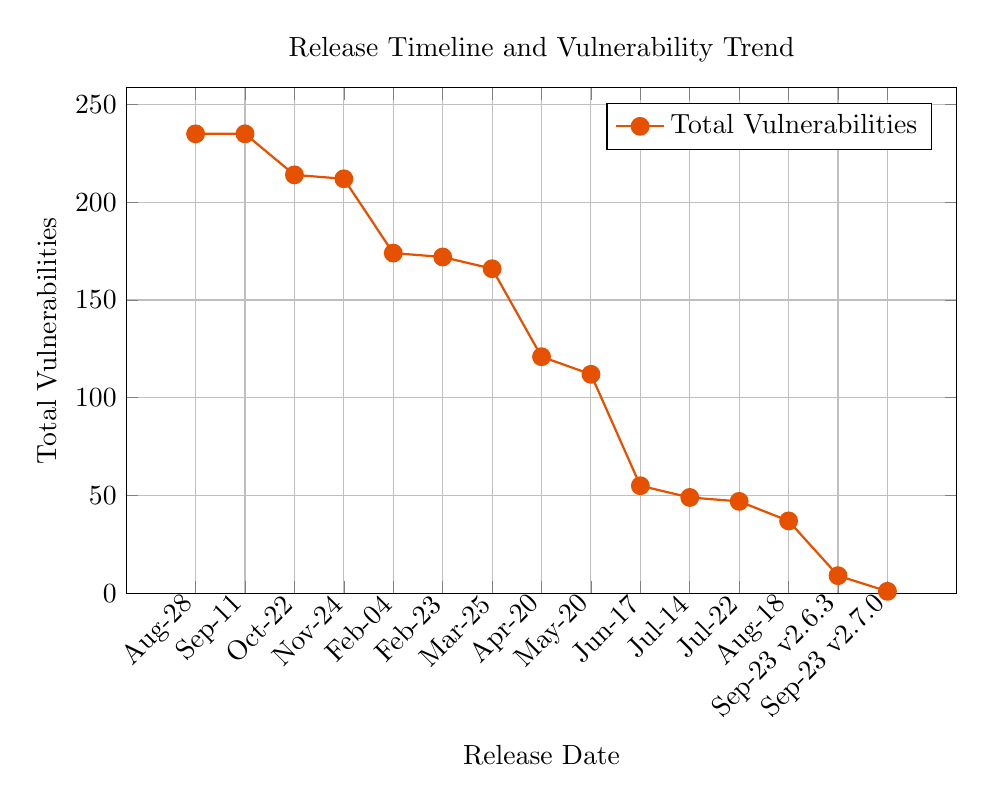
\begin{tikzpicture}
        \begin{axis}[
            title={Release Timeline and Vulnerability Trend},
            xlabel={Release Date},
            ylabel={Total Vulnerabilities},
            symbolic x coords={Aug-28,Sep-11,Oct-22,Nov-24,Feb-04,Feb-23,Mar-25,Apr-20,May-20,Jun-17,Jul-14,Jul-22,Aug-18,{Sep-23 v2.6.3},{Sep-23 v2.7.0}},
            xtick=data,
            x tick label style={rotate=45,anchor=east},
            legend pos=north east,
            grid=major,
            width=\textwidth,
            height=8cm,
            ymin=0,
        ]
        \addplot[color=SeverityHigh,thick,mark=*,mark size=3pt] coordinates {
            (Aug-28,235) (Sep-11,235) (Oct-22,214) (Nov-24,212) (Feb-04,174) (Feb-23,172) (Mar-25,166) (Apr-20,121) (May-20,112) (Jun-17,55) (Jul-14,49) (Jul-22,47) (Aug-18,37) ({Sep-23 v2.6.3},9) ({Sep-23 v2.7.0},1)
        };
        \legend{Total Vulnerabilities}
        \end{axis}
    \end{tikzpicture}
    \caption{Release frequency and vulnerability reduction over time}
    \label{fig:timeline}
\end{figure}

The timeline reveals a consistent release cadence averaging $\sim$28 days across the 2.5.x and 2.6.x series, punctuated by faster turnarounds when warranted: v2.6.1 shipped just 8 days after v2.6.0. The most striking entry is the tail: \textbf{v2.6.3 and v2.7.0 were published on the same day} (2026-09-23, roughly half an hour apart). This is a deliberate pattern rather than an anomaly --- v2.6.3 is the final patch of the 2.6 line, carrying the Alpine 3.24.2 rebase to users who must stay on 2.6.x, while v2.7.0 opens the new minor line with the full set of application fixes. Users on either track receive the OS-layer cleanup; only those who move to 2.7.0 also clear the OpenBao core advisories.

\section{Glossary of Security Terms}
\begin{description}
    \item[CVE (Common Vulnerabilities and Exposures):] A list of publicly disclosed computer security flaws. Each entry (e.g., CVE-2024-1234) represents a specific vulnerability in a software package.
    \item[CVSS (Common Vulnerability Scoring System):] A free and open industry standard for assessing the severity of computer system security vulnerabilities. Scores range from 0 to 10.
    \item[Severity Levels:] 
    \begin{itemize}
        \item \textbf{Critical:} Vulnerabilities that could be easily exploited by a remote attacker to gain full control of the system.
        \item \textbf{High:} Vulnerabilities that are difficult to exploit but could result in significant elevated privileges or data loss.
        \item \textbf{Medium:} Vulnerabilities that require specific configurations or local access to exploit.
        \item \textbf{Low:} Vulnerabilities that have very little impact on the system's security.
    \end{itemize}
    \item[OCI Image (Open Container Initiative):] A standard for container images that ensures portability across different container engines (like Docker or Podman).
    \item[Trivy:] An open-source vulnerability scanner specifically designed for containers and other artifacts.
\end{description}

\section{Conclusion}
The analysis indicates that OpenBao has undergone sustained and substantial security hardening. Moving from version 2.4.0 to the latest 2.7.0 release reduces the vulnerability count from 235 to a single finding --- a \textbf{99.6\% reduction} --- and eliminates every Critical, High, Medium and Low-severity item, yielding a perfect 100.0/100 weighted Security Posture Score.

Two distinct forces produced that result, and the data separates them cleanly. The \textbf{operating-system layer} was cleared by disciplined base-image maintenance: all fifteen analyzed releases shipped the newest Alpine patch available on their build date, and the Alpine 3.24.2 rebase in v2.6.3 removed the last 20 OS findings in one step. The \textbf{application layer} was cleared by upstream code fixes: v2.7.0 retires the seven OpenBao core advisories --- five HIGH, two MEDIUM --- that had persisted in all fourteen prior releases. Neither improvement alone would have been sufficient; together they leave only GO-2026-5932, an advisory on the deprecated \texttt{golang.org/x/crypto/openpgp} package that carries no fix and no severity score.

\textbf{OpenBao's adherence to Semantic Versioning and its low-risk minor release strategy} --- similar to PostgreSQL's versioning philosophy --- ensures that upgrading to the latest minor version is not only safe but actively recommended. The v2.6.3/v2.7.0 pairing illustrates the point precisely: both shipped on 2026-09-23, with v2.6.3 delivering the base-image cleanup to users pinned to the 2.6 line and v2.7.0 delivering both that cleanup and the application fixes. The project supports conservative upgraders without holding back those who move forward.

One methodological caveat deserves emphasis. Every version's counts in this edition are \textbf{higher} than in the previous report (v2.6.1 moved from 10 to 47 findings, v2.5.5 from 15 to 55) purely because this rescan used a Trivy database four months newer. No image changed; the set of known CVEs did. This is why all fifteen tags are rescanned in a single session against one shared database, and it is a reminder that an absolute vulnerability count is only meaningful alongside the date and database that produced it. Relative comparisons within this report remain valid; comparisons against externally published figures generally do not.

Organizations running older minor versions should prioritize upgrading to \textbf{v2.6.3 or later}, and to v2.7.0 where the minor bump is acceptable. This rescan places v2.5.2 through v2.5.4 in the MEDIUM risk band and everything earlier in the HIGH band, while v2.5.5 onward sits in LOW. As demonstrated throughout, staying on an outdated minor version exposes systems to substantially higher risk than the minimal effort a minor upgrade requires.

\end{document}
